\documentclass{article}

\usepackage{graphicx}
\usepackage{tikz}
\usepackage{tikzsymbols}
\usetikzlibrary{calc,patterns,shapes.geometric}
\pagestyle{empty}
\usepackage[margin=0pt]{geometry}
\geometry{papersize={14in,12in}}

\def\centerarc[#1](#2)(#3:#4:#5){\draw[#1] ($(#2)+({#5*cos(#3)},{#5*sin(#3)})$) arc (#3:#4:#5);}

\begin{document}
	\begin{figure}
		\centering
		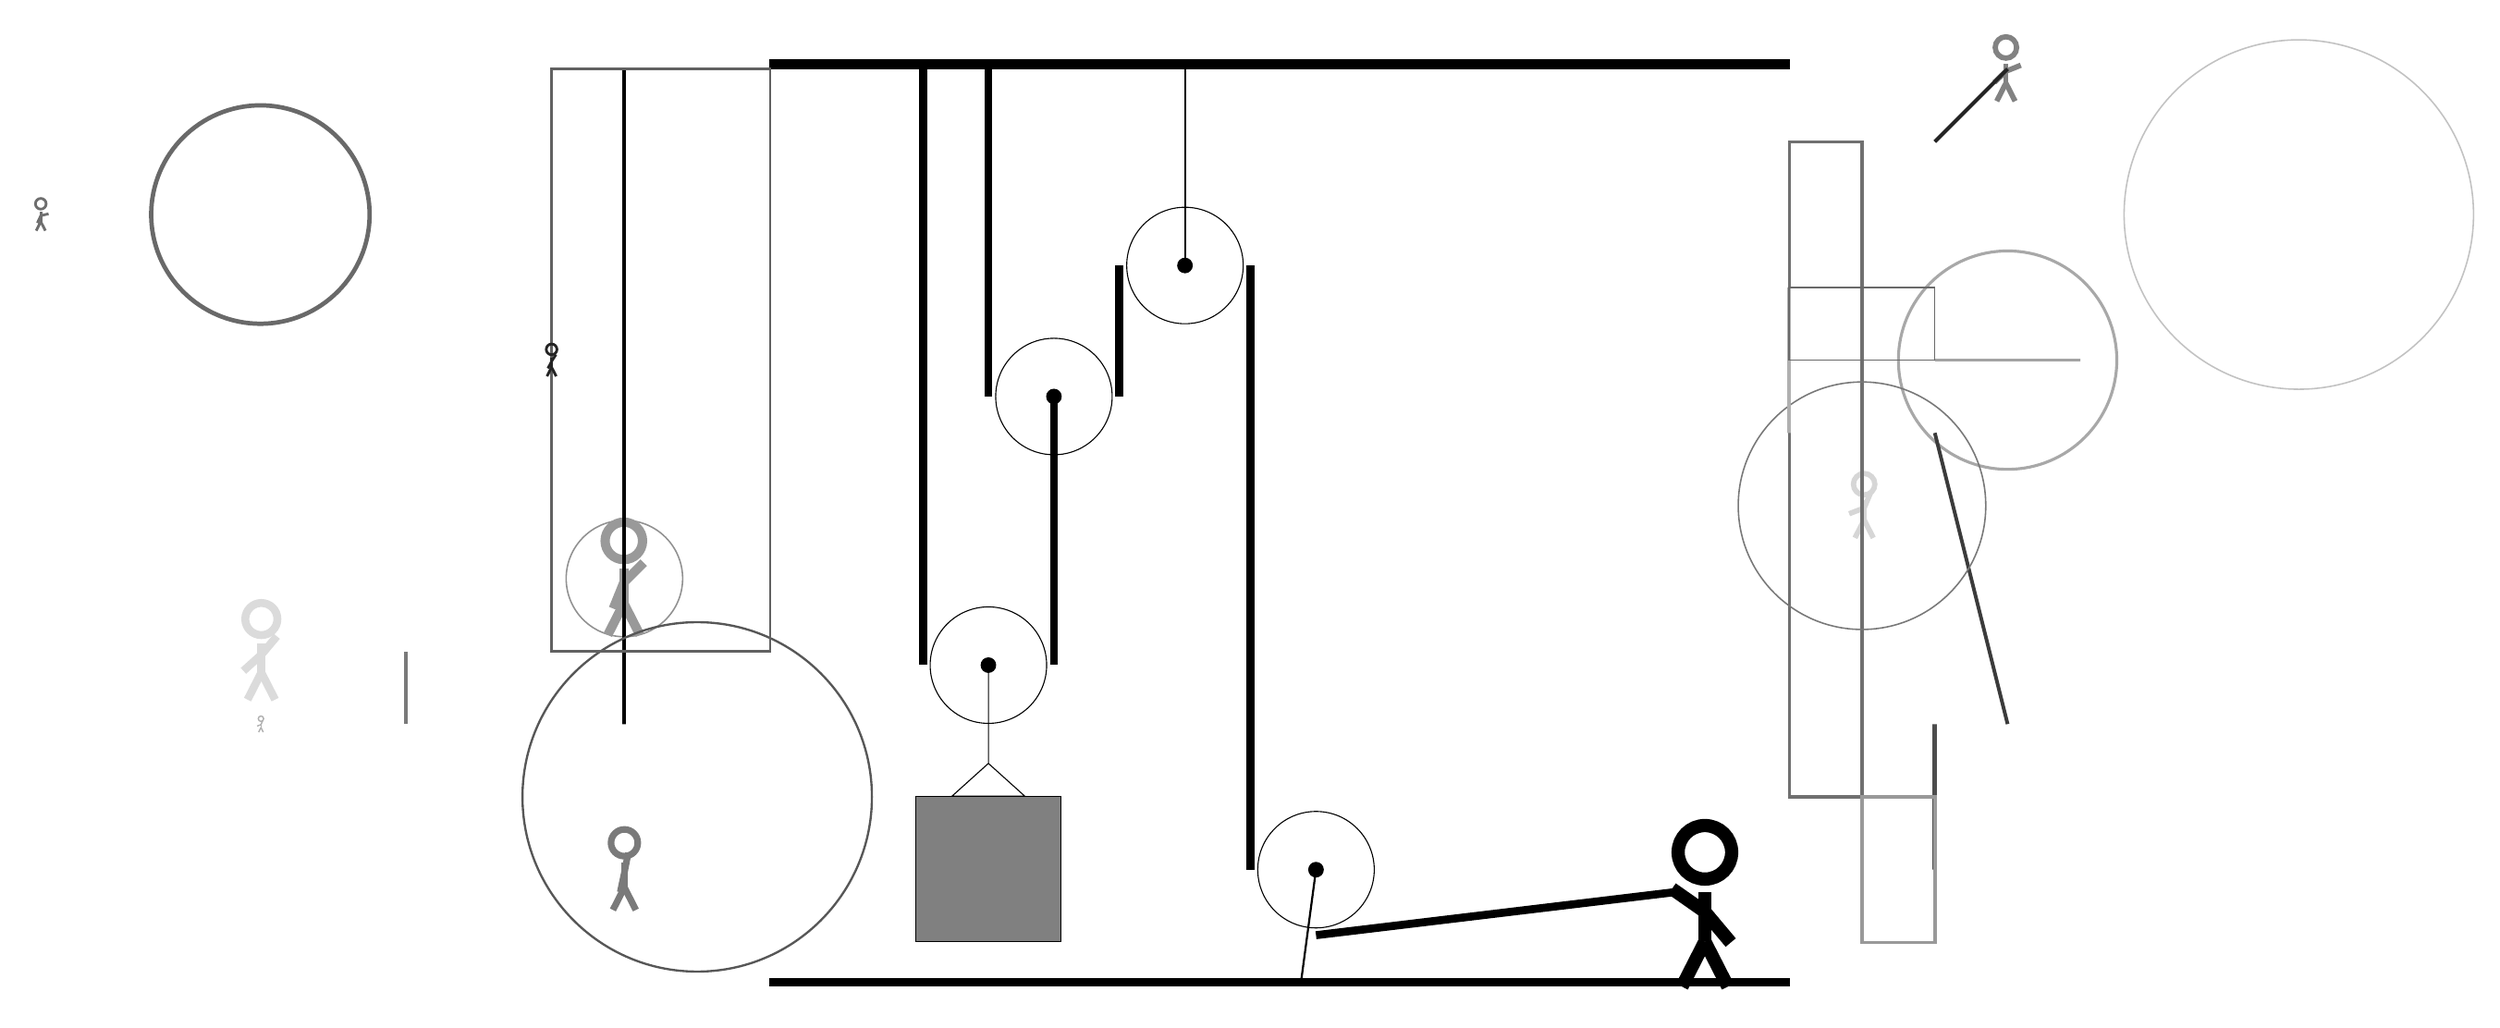
\begin{tikzpicture}
			%%%%% START %%%%%
			
			\draw[fill=black] (-2, 9) rectangle (12, 9.125);
			
			\draw (1, 0.81) circle (0.8);
			\draw[fill=black] (1, 0.81) circle (0.1);
			
			\draw (1.9, 4.5) circle (0.8);
			\draw[fill=black] (1.9, 4.5) circle (0.1);
			
			\draw (3.7, 6.3) circle (0.8);
			\draw[fill=black] (3.7, 6.3) circle (0.1);
			\draw[thick] (3.7, 6.3) -- (3.7, 9);
			
			\draw [line width=0.2mm, color=black!24](19, 7) circle (2.4);
			
			\draw [line width=0.4mm, color=black!34](15, 5) circle (1.5);
			\draw [line width=0.2mm, color=black!43](-4, 2) circle (0.8);
			\draw[line width=0.5mm, color=black!77](14, 4) -- (15, 0);
			
			\node[line width=0.2mm, color=black!40] at (-4, 2) {\Strichmaxerl[7][68][45]};
			
			\draw[line width=0.5mm, color=black!100] (-4, 0) rectangle (-4, 9);
			\node[line width=0.2mm, color=black!31] at (-9, 0) {\Strichmaxerl[1][20][67]};
			
			\draw [line width=0.3mm, color=black!66](-3, -1) circle (2.4);
			\node[line width=0.2mm, color=black!49] at (15, 9) {\Strichmaxerl[4][44][22]};
			\draw[line width=0.5mm, color=black!52](-7, 0) -- (-7, 1);
			\draw [line width=0.6mm, color=black!59](-9, 7) circle (1.5);
			
			\draw[line width=0.6mm, color=black!70] (14, -2) rectangle (14, 0);
			\draw[line width=0.3mm, color=black!62] (-2, 1) rectangle (-5, 9);
			
			\node[line width=0.6mm, color=black!16] at (13, 3) {\Strichmaxerl[4][21][67]};
			\draw[line width=0.5mm, color=black!86](14, 8) -- (15, 9);
			\node[line width=0.3mm, color=black!52] at (-4, -2) {\Strichmaxerl[5][78][79]};
			
			\draw[line width=0.4mm, color=black!36] (14, 5) rectangle (16, 5);
			\draw[line width=0.4mm, color=black!56] (13, -1) rectangle (12, 8);
			\draw [line width=0.2mm, color=black!53](13, 3) circle (1.7);
			\draw[line width=0.5mm, color=black!31] (12, 6) rectangle (12, 4);
			\node[line width=0.4mm, color=black!86] at (-5, 5) {\Strichmaxerl[2][63][57]};
			
			\node[line width=0.2mm, color=black!57] at (-12, 7) {\Strichmaxerl[2][65][14]};
			
			\draw[line width=0.2mm, color=black!59] (12, 5) rectangle (14, 6);
			\node[line width=0.7mm, color=black!14] at (-9, 1) {\Strichmaxerl[6][42][50]};
			\draw[line width=0.5mm, color=black!40] (13, -1) rectangle (14, -3);
			
			\draw (5.5, -2) circle (0.8);
			\draw[fill=black] (5.5, -2) circle (0.1);
			\draw[thick] (5.5, -2) -- (5.3, -3.5);
			
			\draw (1, 0.81) -- (1, -0.54) -- (0.5, -0.99) -- (1.5, -0.99) -- (1, -0.54);
			\draw[fill=black!50] (0, -0.99) rectangle (2, -2.99);
			\draw[line width=1.1mm] (0.1, 9) -- (0.1, 0.81);
			\centerarc[line width=1.1mm](1, 0.81)(180:360:0.9);
			\draw[line width=1.1mm](1.9, 0.81) -- (1.9, 4.5);
			\draw[line width=1.1mm] (1.0, 9) -- (1.0, 4.5);
			\centerarc[line width=1.1mm](1.9, 4.5)(180:360:0.9);
			\draw[line width=1.1mm](2.8, 4.5) -- (2.8, 6.3);
			\centerarc[line width=1.1mm](3.7, 6.3)(0:180:0.9);
			\draw[line width=1.1mm] (4.6, 6.3) -- (4.6, -2);
			\centerarc[line width=1.1mm](5.5, -2)(0:90:-0.9);
			\draw[line width=1.1mm](5.5, -2.9) -- (10.5, -2.3);
			
			\node at (10.8, -2.5) {\Strichmaxerl[10][-35][-50]};
			
			\draw[fill=black] (-2, -3.5) rectangle (12, -3.6);
			
			%%%%% END %%%%%
		\end{tikzpicture}
	\end{figure}	
\end{document}